
\section{Numerical modelling using \textit{Apollo Blastsimulator}}
\subsection{Mesh sensitivity}
A mesh sensitivity study was undertaken to inform the choice of mesh to be used to generate the datasets herein. 
The lower bound of the dataset was chosen as this represents the highest required resolution.
Table \ref{tab:mesh_sens} presents the meshes that were studied.

A feature of \textit{Apollo blastsimulator} is its dynamic mesh adaptation (DMA) capabilities (Figure \ref{fig:DMA}).
This allows the efficient use of computational resources by directing them to areas within the mesh with the largest local gradients (e.g. the shock front).
DMA was used to generate the data within this research, and its effects are studied compared with the uniform mesh resolution scenario.

\begin{figure}[htpb]
	\centering
	\includegraphics[scale=0.75, keepaspectratio]{Images/local_mesh_dma.pdf}
	\caption{Dynamic mesh adaptation in \textit{Apollo blastsimulator}}
	\label{fig:DMA}
\end{figure}

\begin{table}
	\begin{subtable}{0.45\textwidth}
		\centering
		\caption{Ultimate cell length (mm) for meshes used.\linebreak}
		\import{Tables/}{z0_055_mesh_mm.tex}
	\end{subtable}
	\hspace{5mm}
	\begin{subtable}{0.45\textwidth}
		\centering
		\caption{Number of cells in distance between charge centre and measuring location (at 0$^{\circ}$ angle of incidence).}	
		\import{Tables/}{z0_055_mesh_R.tex}
	\end{subtable}
	\caption{Mesh sensitivity study information for z = 0.11$m/kg^{\frac{1}{3}}$.}
	\label{tab:mesh_sens}
\end{table}

\begin{figure}[htpb]
	 \centering
	 \includegraphics{Graphs/mesh_convergence_z0_055_1.pdf}
	 \caption{Mesh convergence study for z = 0.108$m/kg^{\frac{1}{3}}$}
	 \label{fig:mesh_convergence_z0_055_1}
\end{figure}
Figure \ref{fig:mesh_convergence_z0_055_1} presents the mesh convergence data as a function of number of cells between the centre of the charge and the target face. 
Convergence was deemed to be adequate within $10\%$ of the ``convereged'' value at $R/\text{cell length} = 15$. 
Convergence is shown to be quicker when considering the total impulse on a $1m^2$ plate.

Further mesh studies were performed to assess the impact of the DMA module, and different $R/\text{cell length}$ values on the distribution of peak specific impulse. 
Figure \ref{fig:mesh_convergence_dataset2} presents this information, with the plot labels representing the meshes in Table \ref{tab:mesh_sens2}. 
It shows that overall, the distribution itself convergences at a fairly coarse level (ultimate cell size of $6.250$mm), whilst it is only the peak values that do not converge for the coarser meshes, shown in Figure \ref{fig:mesh_convergence_dataset3}.
Meshes E and F study the effect of the DMA module on the overall distribution. 
It is shown that the DMA does introduce artificial oscillations to the impulse distribution, however, in context with the shape of the overall profile these are deemed to be acceptable. 
Mesh D was chosen, with an ultimate cell size of $3.15mm$.
\begin{table}[htpb]
	\centering
	\caption{Information for mesh strategy in context of range of scaled distance ($0.1 \leq z \leq 0.2m/kg^{\frac{1}{3}}$).}	
	\import{Tables/}{dataset_meshes.tex}
	\label{tab:mesh_sens2}
\end{table}

\begin{figure}[htpb]
	\begin{subfigure}{0.4\textwidth}
		\centering
		\includegraphics{Graphs/mesh_convergence_dataset2.pdf}
		\caption{Specific impulse distribution for z $= 0.187m/kg^{\frac{1}{3}}$ for DMA analysis.}
		\label{fig:mesh_convergence_dataset2}
	\end{subfigure}
	\begin{subfigure}{0.4\textwidth}
	\centering
	\includegraphics{Graphs/mesh_convergence_dataset3.pdf}
	\caption{Total area integrated impulse impinging on a $1m^2$ target plate for each mesh.}
	\label{fig:mesh_convergence_dataset3}
	\end{subfigure}	
	\caption{Mesh strategy across dataset range.}
\end{figure}

\subsection{Experimental validation}
\textit{Apollo blastsimulator} was validated against available experimental data published in \cite{rigbyExperimentalMeasurementSpecific2019}. 
Here 100g spherical PE4 chargers were detonated at a perpendicular standoff distances of 80mm and 380mm (to the centre of the charge).
Three tests were performed in total, with 17 HPBs in each test: one located in the centre of the target; four at 25 mm from the centre; four at 50 mm from the centre; four at 75 mm from the centre; and four at 100 mm from the centre. 
These correspond to angles of incidence of: $0, 17, 32, 43 \text{ and } 51$ degrees.
The comparison for pressure and impulse time-histories are given in Figure \ref{fig:80mm_validation_OP_imp}.
Pressure-time histories show good agreement for peak values and arrival times, whilst the impulse time-histories show fairly good agreement for all given angles of incidence. 

An experimental comparison for peak impulse distribution is shown in Figure \ref{fig:mesh_80mm_va} where \textit{Apollo} appears to agree with the upper bound of the experimental dataset. 

\begin{figure}[htpb]
	\begin{subfigure}{\linewidth}
		\centering
		\includegraphics{Graphs/80mm_validation.pdf}
		\caption{0 degrees}
		\label{fig:80mm_validation}
	\end{subfigure}
	\begin{subfigure}{\linewidth}
		\centering
		\includegraphics{Graphs/80mm_validation_a.pdf}
		\caption{17 degrees}
		\label{fig:80mm_validation_a}
	\end{subfigure}
	\begin{subfigure}{\linewidth}
		\centering
		\includegraphics{Graphs/80mm_validation_b.pdf}
		\caption{32 degrees}
		\label{fig:80mm_validation_b}
	\end{subfigure}
	\begin{subfigure}{\linewidth}
		\centering
		\includegraphics{Graphs/80mm_validation_c.pdf}
		\caption{43 degrees}
		\label{fig:80mm_validation_c}
	\end{subfigure}
	\begin{subfigure}{\linewidth}
		\centering
		\includegraphics{Graphs/80mm_validation_d.pdf}
		\caption{51 degrees}
		\label{fig:80mm_validation_d}
	\end{subfigure}
	\caption{Experimental validation for overpressure and impulse time histories at z=0.17 $m/kg^{\frac{1}{3}}$ for various angles of incidence.}
	\label{fig:80mm_validation_OP_imp}
\end{figure}

\begin{figure}[htpb]
	\begin{subfigure}{\linewidth}
		\centering
		\includegraphics{Graphs/n80mm_validation.pdf}
		\caption{0 degrees}

	\end{subfigure}
	\begin{subfigure}{\linewidth}
		\centering
		\includegraphics{Graphs/n80mm_validation_a.pdf}
		\caption{17 degrees}

	\end{subfigure}
	\begin{subfigure}{\linewidth}
		\centering
		\includegraphics{Graphs/n80mm_validation_b.pdf}
		\caption{32 degrees}

	\end{subfigure}
	\begin{subfigure}{\linewidth}
		\centering
		\includegraphics{Graphs/n80mm_validation_c.pdf}
		\caption{43 degrees}

	\end{subfigure}
	\begin{subfigure}{\linewidth}
		\centering
		\includegraphics{Graphs/n80mm_validation_d.pdf}
		\caption{51 degrees}

	\end{subfigure}
	\caption{Experimental validation for overpressure and impulse time histories at z=0.17 $m/kg^{\frac{1}{3}}$ for various angles of incidence.}

\end{figure}

\begin{figure}[htpb]
	\begin{subfigure}{0.45\linewidth}
		\centering
		\includegraphics{Graphs/mesh_80mm_val.pdf}
		\caption{100g PE4 sphere at 80mm standoff, z = 0.16$m/kg^{\frac{1}{3}}$.}
		\label{fig:mesh_80mm_val}
	\end{subfigure}
	\begin{subfigure}{0.45\linewidth}
		\centering
		\includegraphics{Graphs/mesh_380mm_val.pdf}
		\caption{380mm standoff, z = 0.77$m/kg^{\frac{1}{3}}$.}
		\label{fig:mesh_380mm_val}
	\end{subfigure}
\end{figure}

Considering the dataset as a whole, the peak specific impulse distributions are shown in Figure \ref{fig:mesh_convergence_dataset1}, and smoothed versions in Figure \ref{fig:mesh_convergence_dataset1a}. 
The smoothing was completed with a Savitzky-Golay filter \cite{savitzkySmoothingDifferentiationData1964} and is shown to maintain the overall distribution whilst removing the artificial oscillations from the DMA module. 
Normalising each sample to the maximum at theta $= 0$ is shown in Figure \ref{fig:mesh_convergence_dataset1b} where it is shown that the normalised specific impulse profiles across the chosen range of scaled distances can be considered homogeneous.
